\documentclass[a4paper, 12pt]{article}

%%% Работа с русским языком
\usepackage{cmap}					% поиск в PDF
\usepackage{mathtext} 				% русские буквы в формулах
\usepackage[T2A]{fontenc}			% кодировка
\usepackage[utf8]{inputenc}			% кодировка исходного текста
\usepackage[russian]{babel}	% локализация и переносы

%%% Дополнительная работа с математикой
\usepackage{amsmath,amsfonts,amssymb,amsthm,mathtools} % AMS
\usepackage{icomma} % "Умная" запятая: $0,2$ --- число, $0, 2$ --- перечисление

%% Номера формул
%\mathtoolsset{showonlyrefs=true} % Показывать номера только у тех формул, на которые есть \eqref{} в тексте.

%% Шрифты
\usepackage{euscript}	 % Шрифт Евклид
\usepackage{mathrsfs} % Красивый матшрифт

%% Поля
\usepackage[left=2cm,right=2cm,top=2cm,bottom=2cm,bindingoffset=0cm]{geometry}

%% Русские списки
\usepackage{enumitem}
\makeatletter
\AddEnumerateCounter{\asbuk}{\russian@alph}{щ}
\makeatother

%%% Работа с картинками
\usepackage{graphicx}  % Для вставки рисунков
\graphicspath{{images/}{images2/}}  % папки с картинками
\setlength\fboxsep{3pt} % Отступ рамки \fbox{} от рисунка
\setlength\fboxrule{1pt} % Толщина линий рамки \fbox{}
\usepackage{wrapfig} % Обтекание рисунков и таблиц текстом

%%% Работа с таблицами
\usepackage{array,tabularx,tabulary,booktabs} % Дополнительная работа с таблицами
\usepackage{longtable}  % Длинные таблицы
\usepackage{multirow} % Слияние строк в таблице

%% Красная строка
\setlength{\parindent}{2em}

%% Интервалы
\linespread{1}
\usepackage{multirow}

%% TikZ
\usepackage{tikz}
\usetikzlibrary{graphs,graphs.standard}

%% Верхний колонтитул
\usepackage{fancyhdr}
\pagestyle{fancy}

%% Перенос знаков в формулах (по Львовскому)
\newcommand*{\hm}[1]{#1\nobreak\discretionary{}
	{\hbox{$\mathsurround=0pt #1$}}{}}

%% Мои дополнения
\usepackage{float} %Добавляет возможность работы с командой [H] которая улучшает расположение на странице
\usepackage{gensymb} %Красивые градусы
\usepackage{graphicx}               % Импорт изображений
\usepackage{caption} % Пакет для подписей к рисункам, в частности, для работы caption*

% подключаем hyperref (для ссылок внутри  pdf)
\usepackage[unicode, pdftex]{hyperref}

%%% Теоремы
\theoremstyle{plain}                    % Это стиль по умолчанию, его можно не переопределять.
\renewcommand\qedsymbol{$\blacksquare$} % переопределение символа завершения доказательства

\newtheorem{theorem}{Теорема}[section] % Теорема (счетчик по секиям)
\newtheorem{proposition}{Утверждение}[section] % Утверждение (счетчик по секиям)
\newtheorem{definition}{Определение}[section] % Определение (счетчик по секиям)
\newtheorem{corollary}{Следствие}[theorem] % Следстиве (счетчик по теоремам)
\newtheorem{problem}{Задача}[section] % Задача (счетчик по секиям)
\newtheorem*{remark}{Примечание} % Примечание (можно переопределить, как Замечание)
\newtheorem{lemma}{Лемма}[section] % Лемма (счетчик по секиям)

\begin{document}
    \newcommand{\HRule}{\rule{\linewidth}{0.7mm}} % Defines a new command for the horizontal lines, change thickness here
	
	\begin{center}
		\large\textbf{Московский Физико-Технический Институт}\\ % Name of your university/college
		\large\textbf{(государственный университет)}
	
		\vfill
		
		\Large Лабораторная работа по курсу общей физики № *labnum*\\[0.5cm] % Preambule of your document title
		
		
		\HRule
		\\[0.4cm]
		{ \huge \bfseries *name of your labwork*}% Title of your document
		\\[0.4cm] 
		\HRule
		\\[0.5cm]
		
		\ \\
	\textbf{\large Автор:} \\	
	\large *your name* *groupname*\\ % Your name and something more, your group num for example
		\vfill
		\hspace*{-0.8 cm}
\includegraphics[width=100 pt]{frkt_logo}\\ % logo of your  company/university/college
		\large Долгопрудный, 2021 % location and year
	\end{center}

\newpage
\setcounter{page}{2}
\fancyfoot[c]{\thepage}
\fancyhead[L] {Работа № *labnum*} % some information in page header
\fancyhead[R]{}

    \section*{Теоретическая часть}

    Гамма-лучи возникают при переходе возбужденных ядер из одного энергетического состояния в другое, более низкое. Энергия $\gamma$-квантов обычно заключена между несколькими десятками килоэлектронвольт и несколькими миллионами электрон-вольт. Гамма-кванты не несут электрического заряда, их масса равна нулю. Проходя, через вещество, пучок $\gamma$-квантов постепенно ослабляется. Ослабление просходит по експоненциальному закону, который может быть записан в следующей форме:
	\begin{equation}
		\label{eq1}
		I = I_0 e^{-\mu l}, \quad I_o e^{-\mu 'm_1} 
	\end{equation}

	В этих формулах $I, I_0$ -- интенсивности прошедшего и падающего излучений, $l$ -- длина пути, пройденного пучком $\gamma$-лучей, $m_1$ --
	масса пройденного вещества, приходящаяся на единицу площади, $\mu$ и
	$ \mu' $ -- константы, величина которых зависит от вещества, сквозь кото-
	рое проходят $\gamma$-лучи.
	
	Ослабление потока $\gamma$-лучей, происходящее при прохождении среды, связано с тремя эффектами: 
    
    \begin{enumerate}
        \item фотоэлектрическим поглощением
        \item комптоновским рассеянием
        \item генерацией электрон-позитронных пар
    \end{enumerate}
	
	В случае опытов, поставленных в хорошей геометрии, при прохождении $\gamma$-лучей через вещество меняет только количество, но не энергия $\gamma$-квантов в пучке, так что коэффициент $\mu$, характеризующий поглощение $\gamma$-квантов в веществе, не зависит от длины пути. Обозначим через $-dN$ число $\gamma$-квантов, выбывших их пучка на пути $dl$. Это число пропорционально имеющемуся их числу $N$ и пройденному пути $dl$. Cледовательно,
	\begin{equation}
		\label{eq2}
		-dN = \mu N \, dl.
	\end{equation} 
	Интегрируя уравнение~(\ref{eq2}) от нулевой толщины до заданной, получим
	\begin{equation}
		\label{eq3}
		N = N_0 e^{-\mu l}.
	\end{equation}

	Вообще говоря, в плохой геометрии, когда рассеянные под небольшими углами $\gamma$-кванты остаются в пучке, их спектр с прохождением вещества меняется, поэтому формула~(\ref{eq1}) непреминима. Однако в этом случае она работает лучше, чем можно было ожидать.
	
	В данной работе коэффициент ослабления $\mu$ измеряется в хорошей геометрии. Из формулы~(\ref{eq3}) имеем:
	\begin{equation} \label{formula}
		\mu = \frac{1}{l} \ln \frac{N_0}{N}.
	\end{equation}

	Для определения коэффициента ослабления нужно, таким образом, измерить толщтну образца $l$, число падающих частиц $N_0$ и число частиц $N$, прошедших через образец.

    \section*{Эксперементальная установка}

    Схема установки, исползуемой в работе, показана на рис.~\ref{fig:ustanovka1}. Свинцовый коллиматор выделяет узкий почти параллельный пучок $\gamma$-квантов, проходящий через набор поглотителей П и регистрируемый сцинтиляцонным счетчиком. Сигналы от счетчика усиливаются и регистрируются пересчетным прибором ПП. Высоковольтный выпрямитель ВВ обеспечивает питание сцинтилляционного счетчика.
	

    \begin{figure}
        \centering
        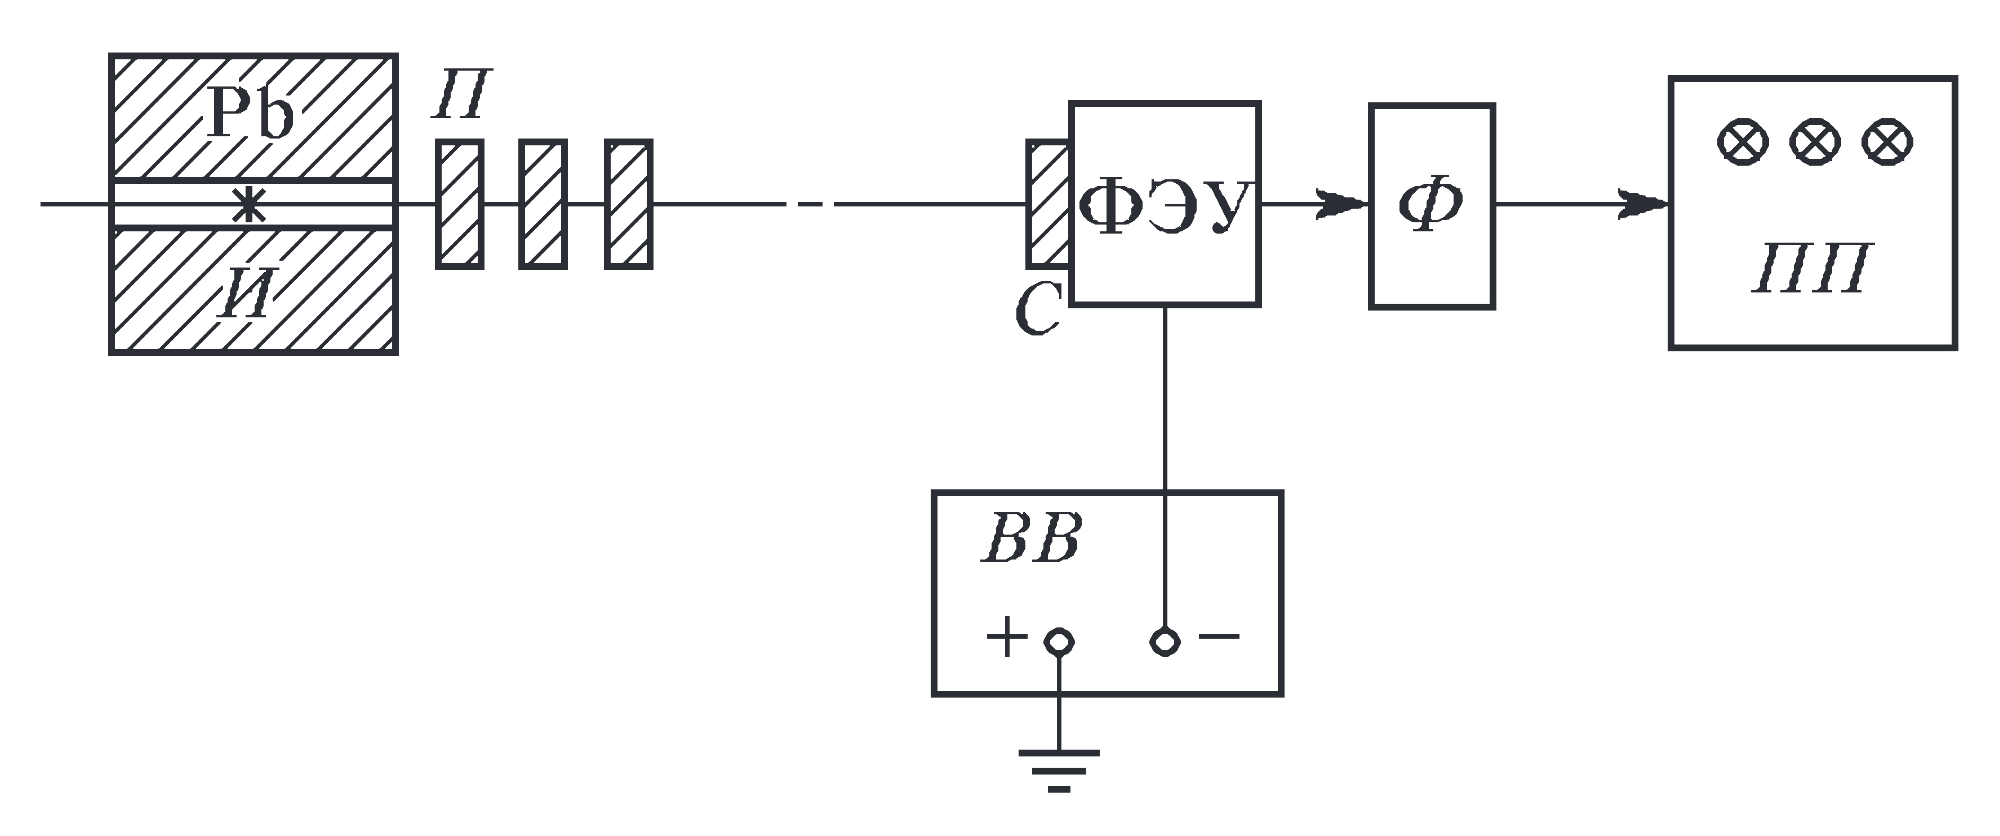
\includegraphics[width=0.7\textwidth]{equipment1.png}
        \caption{Блок-схема установки, используемой для измерения коэффициентов ослабления потока $\gamma$-лучей}
        \label{fig:ustanovka1}
    \end{figure}

    При недостаточно хорошей геометрии в результаты опытов могут вкрасться существенные погрешности. В реальных установках всегда имеется конечная вероятность того, что $\gamma$-квант провзаимодействует в поглотителе несколько раз до того, как попадет в детектор (пути таких квантов показаны на рис.~\ref{fig:ustanovka2}). Чтобы уменьшить число таких случаев, в данной работе сцинтилляционный счетчик расположен на большом расстоянии от источиника $\gamma$-квантов, а поглотители имеют небольшие размеры. Их следует устанавливать за коллиматорной щелью на некотором расстоянии друг от друга, чтобы испытавшие комптоновское рассеяние и выбывшие из прямого потока кванты с меньшей вероятностью могли в него вернуться.

    \begin{figure}
        \centering
        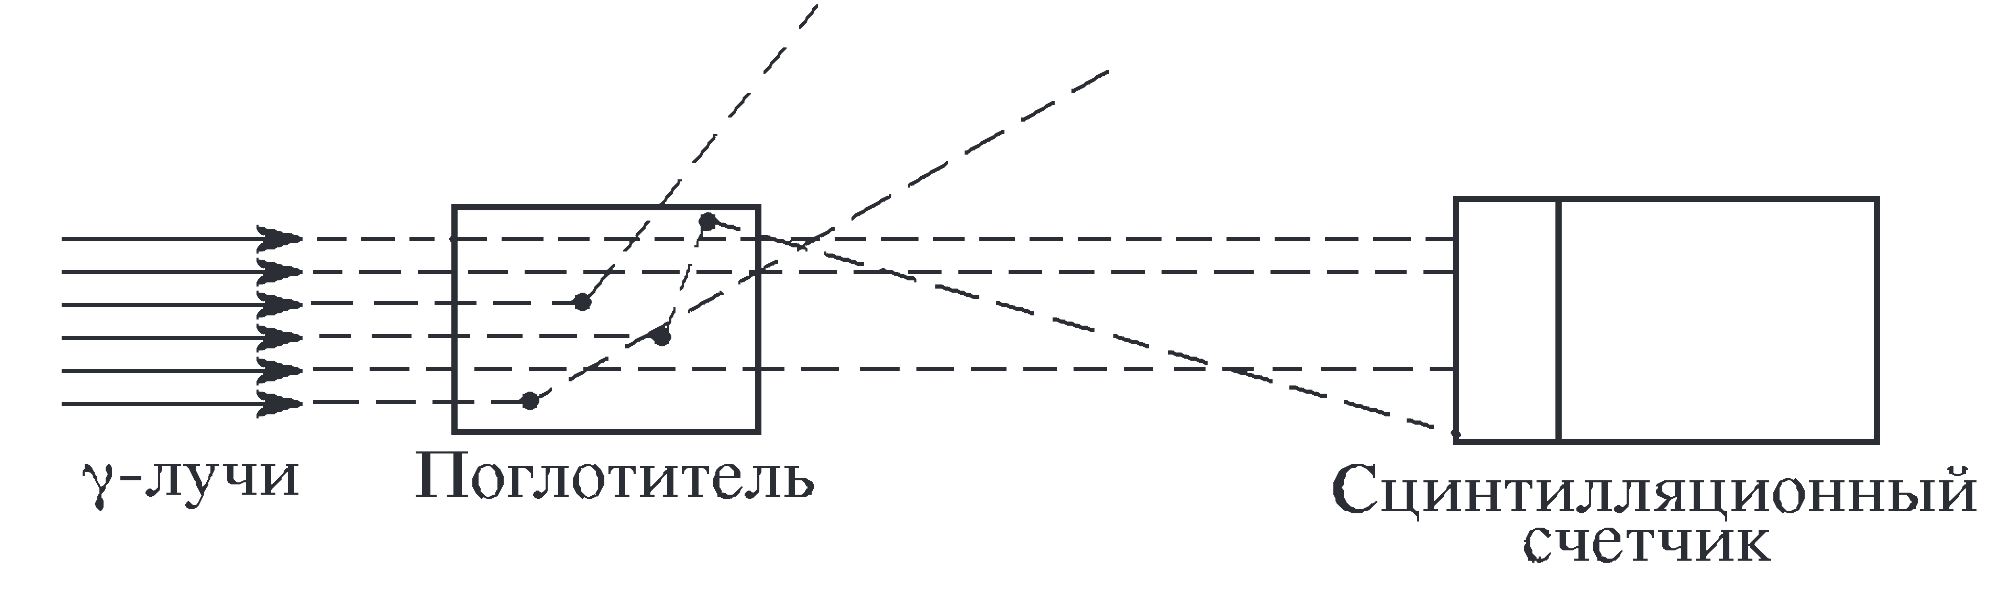
\includegraphics[width=0.7\textwidth]{equipment2.png}
        \caption{Схема рассеяния $\gamma$-квантов в поглотителе}
        \label{fig:ustanovka2}
    \end{figure}

    \section*{Обработка эксперементаьных даннх}

    По условиям эксперемента, точность измерений не должна быть хуже 1 \% для 
    определения фона и не хуже 0.3 \% для всех остальных измерений.

    Вспомним, что погрешность среднего соотносится с погрешностью отдельного измерения как

    \begin{equation*}
        \sigma_{\overline{x}} = \frac{\sigma_x}{\sqrt{N}}
    \end{equation*}

    где $N$ -- число измерений. Тогда относительная погрешность измерений $\varepsilon$:

    \begin{equation*}
        \varepsilon \sim \frac{1}{\sqrt{N}}
    \end{equation*}

    Из этих соображений, получаем, чтобы получить точность не хуже чем 1 \% необходимо
    регистрировать не менее 10000 частиц, чтобы получить точность не хуже 0.3 \% необходимо
    регистрировать не менее 100000 частиц.

    В условиях нашего эксперемента необходимо учитывать фоновое излучение. Поэтому введем обозначения:

    \[ N = n - n_{\text{фон}} ~~~ N_0 = n_0 - n_{\text{фон}} \]

    Кроме того, в процессе вычислений мы будем брать количество частиц, зарегистрированных в секунду.
    Поэтому, введем обозначения: $N$ -- количество частиц, зарегистрированных за промежуток времени $t$,
    $N' = N / t$ -- количество частиц, зарегистрированных в секунду.

    \begin{center}
        $n_{\text{фон}} = 10015$ (за 100 с) \\
        $n_0 = 291115$ (за 10 с)
    \end{center}

    \begin{table}[h!]
    \centering
    \begin{tabular}{|c|c|c|c|}
    \hline
    Алюминий            & Железо               & Свинец               & Пробка              \\ \hline
    (20 $\pm$ 0.05) мм  & (10 $\pm$ 0.05) мм   & (4.8 $\pm$ 0.05) мм  & (20 $\pm$ 0.05) мм  \\ \hline
    \end{tabular}
    \caption{Толщина заглушек для разных материалов}
    \label{tab:materials}
\end{table}

    Таблица исходных данных \ref{tab:data}. Будем считать, что погрешность измерения частиц $\sqrt{N'}$.
    \begin{table}[]
    \centering
    \begin{tabular}{|ll|ll|ll|}
    \hline
    \multicolumn{2}{|l|}{4 В}                                      & \multicolumn{2}{l|}{6 В}                                     & \multicolumn{2}{l|}{9 В}                                     \\ \hline
    \multicolumn{1}{|l|}{V$\pm 0.01$, В}    & I $\pm 0.001$ мА     & \multicolumn{1}{l|}{V$\pm 0.01$, В}    & I $\pm 0.001$ мА    & \multicolumn{1}{l|}{V$\pm 0.01$, В}    & I $\pm 0.001$ мА    \\ \hline
    \multicolumn{1}{|l|}{4.25}              & 0.062                & \multicolumn{1}{l|}{2.60}              & 0.019               & \multicolumn{1}{l|}{5.28}              & 0.015               \\ \hline
    \multicolumn{1}{|l|}{6.25}              & 0.094                & \multicolumn{1}{l|}{6.05}              & 0.066               & \multicolumn{1}{l|}{10.0}              & 0.090               \\ \hline
    \multicolumn{1}{|l|}{8.14}              & 0.127                & \multicolumn{1}{l|}{9.12}              & 0.120               & \multicolumn{1}{l|}{12.6}              & 0.133               \\ \hline
    \multicolumn{1}{|l|}{10.8}              & 0.171                & \multicolumn{1}{l|}{12.3}              & 0.169               & \multicolumn{1}{l|}{14.9}              & 0.167               \\ \hline
    \multicolumn{1}{|l|}{14.6}              & 0.223                & \multicolumn{1}{l|}{16.0}              & 0.221               & \multicolumn{1}{l|}{17.4}              & 0.203               \\ \hline
    \multicolumn{1}{|l|}{17.5}              & 0.258                & \multicolumn{1}{l|}{16.7}              & 0.228               & \multicolumn{1}{l|}{19.5}              & 0.228               \\ \hline
    \multicolumn{1}{|l|}{17.9}              & 0.262                & \multicolumn{1}{l|}{17.4}              & 0.239               & \multicolumn{1}{l|}{20.7}              & 0.235               \\ \hline
    \multicolumn{1}{|l|}{18.7}              & 0.269                & \multicolumn{1}{l|}{18.1}              & 0.249               & \multicolumn{1}{l|}{21.6}              & 0.236               \\ \hline
    \multicolumn{1}{|l|}{19.7}              & 0.274                & \multicolumn{1}{l|}{19.1}              & 0.258               & \multicolumn{1}{l|}{22.5}              & 0.233               \\ \hline
    \multicolumn{1}{|l|}{21.0}              & 0.274                & \multicolumn{1}{l|}{20.0}              & 0.263               & \multicolumn{1}{l|}{24.0}              & 0.203               \\ \hline
    \multicolumn{1}{|l|}{21.9}              & 0.271                & \multicolumn{1}{l|}{21.0}              & 0.263               & \multicolumn{1}{l|}{24.3}              & 0.183               \\ \hline
    \multicolumn{1}{|l|}{22.3}              & 0.261                & \multicolumn{1}{l|}{21.9}              & 0.257               & \multicolumn{1}{l|}{24.5}              & 0.098               \\ \hline
    \multicolumn{1}{|l|}{22.7}              & 0.251                & \multicolumn{1}{l|}{22.5}              & 0.252               & \multicolumn{1}{l|}{25.2}              & 0.078               \\ \hline
    \multicolumn{1}{|l|}{23.0}              & 0.221                & \multicolumn{1}{l|}{23.2}              & 0.236               & \multicolumn{1}{l|}{26.5}              & 0.071               \\ \hline
    \multicolumn{1}{|l|}{23.3}              & 0.211                & \multicolumn{1}{l|}{23.4}              & 0.221               & \multicolumn{1}{l|}{27.6}              & 0.077               \\ \hline
    \multicolumn{1}{|l|}{24.3}              & 0.213                & \multicolumn{1}{l|}{23.5}              & 0.205               & \multicolumn{1}{l|}{28.8}              & 0.093               \\ \hline
    \multicolumn{1}{|l|}{24.7}              & 0.218                & \multicolumn{1}{l|}{23.8}              & 0.169               & \multicolumn{1}{l|}{29.6}              & 0.112               \\ \hline
    \multicolumn{1}{|l|}{25.4}              & 0.232                & \multicolumn{1}{l|}{24.8}              & 0.144               & \multicolumn{1}{l|}{30.6}              & 0.138               \\ \hline
    \multicolumn{1}{|l|}{26.3}              & 0.249                & \multicolumn{1}{l|}{25.8}              & 0.152               & \multicolumn{1}{l|}{31.6}              & 0.160               \\ \hline
    \multicolumn{1}{|l|}{26.8}              & 0.259                & \multicolumn{1}{l|}{27.7}              & 0.194               & \multicolumn{1}{l|}{33.8}              & 0.207               \\ \hline
    \multicolumn{1}{|l|}{27.6}              & 0.275                & \multicolumn{1}{l|}{29.0}              & 0.220               & \multicolumn{1}{l|}{35.8}              & 0.240               \\ \hline
    \multicolumn{1}{|l|}{28.5}              & 0.293                & \multicolumn{1}{l|}{29.9}              & 0.240               & \multicolumn{1}{l|}{37.0}              & 0.250               \\ \hline
    \multicolumn{1}{|l|}{29.4}              & 0.309                & \multicolumn{1}{l|}{31.9}              & 0.277               & \multicolumn{1}{l|}{38.6}              & 0.255               \\ \hline
    \multicolumn{1}{|l|}{32.1}              & 0.359                & \multicolumn{1}{l|}{33.4}              & 0.306               & \multicolumn{1}{l|}{39.4}              & 0.253               \\ \hline
    \multicolumn{1}{|l|}{33.8}              & 0.389                & \multicolumn{1}{l|}{35.0}              & 0.333               & \multicolumn{1}{l|}{41.1}              & 0.241               \\ \hline
    \multicolumn{1}{|l|}{35.0}              & 0.409                & \multicolumn{1}{l|}{36.9}              & 0.346               & \multicolumn{1}{l|}{42.9}              & 0.229               \\ \hline
    \multicolumn{1}{|l|}{37.3}              & 0.419                & \multicolumn{1}{l|}{39.0}              & 0.347               & \multicolumn{1}{l|}{44.4}              & 0.218               \\ \hline
    \multicolumn{1}{|l|}{38.5}              & 0.419                & \multicolumn{1}{l|}{40.9}              & 0.330               & \multicolumn{1}{l|}{46.4}              & 0.201               \\ \hline
    \multicolumn{1}{|l|}{39.4}              & 0.411                & \multicolumn{1}{l|}{42.9}              & 0.316               & \multicolumn{1}{l|}{48.2}              & 0.196               \\ \hline
    \multicolumn{1}{|l|}{40.5}              & 0.400                & \multicolumn{1}{l|}{44.5}              & 0.308               & \multicolumn{1}{l|}{50.1}              & 0.192               \\ \hline
    \multicolumn{1}{|l|}{40.9}              & 0.395                & \multicolumn{1}{l|}{46.1}              & 0.305               & \multicolumn{1}{l|}{51.7}              & 0.199               \\ \hline
    \multicolumn{1}{|l|}{41.7}              & 0.391                & \multicolumn{1}{l|}{47.7}              & 0.308               & \multicolumn{1}{l|}{52.7}              & 0.204               \\ \hline
    \multicolumn{1}{|l|}{42.7}              & 0.387                & \multicolumn{1}{l|}{49.4}              & 0.317               & \multicolumn{1}{l|}{}                  &                     \\ \hline
    \multicolumn{1}{|l|}{44.5}              & 0.388                & \multicolumn{1}{l|}{51.6}              & 0.330               & \multicolumn{1}{l|}{}                  &                     \\ \hline
    \multicolumn{1}{|l|}{45.2}              & 0.390                & \multicolumn{1}{l|}{53.1}              & 0.343               & \multicolumn{1}{l|}{}                  &                     \\ \hline
    \multicolumn{1}{|l|}{49.4}              & 0.417                & \multicolumn{1}{l|}{56.0}              & 0.370               & \multicolumn{1}{l|}{}                  &                     \\ \hline
    \end{tabular}
    \caption{Таблица эксперементальных данных для трех запирающих напряжений}
    \label{tab:data}
    \end{table}

    Поскольку дальше нам придется работать с величиной $\ln \frac{N_0}{N}$, посчитаем ее погрешность.
    Косвенную погрешность величины $u = f(x, y)$ можно посчитать по формуле

    \[ \sigma_u = \sqrt{(f_x')^2 \cdot \sigma_x^2 + (f_y')^2 \cdot \sigma_y^2} \]

    Тогда для погрешности натурального логарифма получим

    \[ \sigma = \sqrt{\left(\frac{\sigma_{N_0}}{N_0} \right)^2 + \left(\frac{\sigma_{N}}{N} \right)^2} \]

    Однако, вспомним, что относительная погрешность задана нам условиями эксперемента и составляет 0.003 (0.3 \%).
    Поэтому $\sigma \approx 0.0774$.

    Построим графики зависимости величины $\ln \frac{N_0}{N}$ от $l$ (длины пути, пройденного через рассеиватель).
    По наклону прямой найдем величину коэффициента $\mu$ \eqref{formula}.

    \begin{figure}
        \centering
        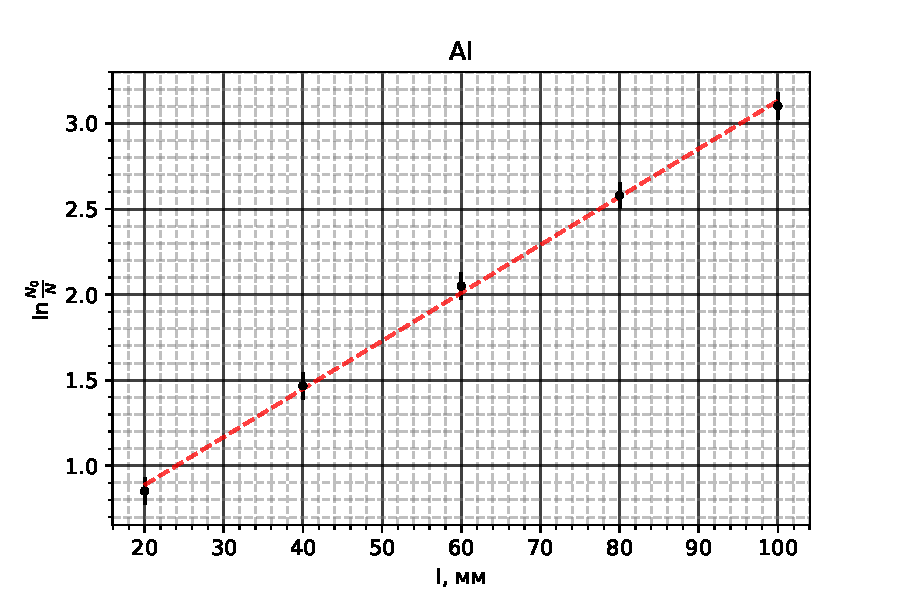
\includegraphics[width=\textwidth]{Al.pdf}
        \caption{График для алюминия}
        \label{fig:Al}
    \end{figure}

    \begin{figure}
        \centering
        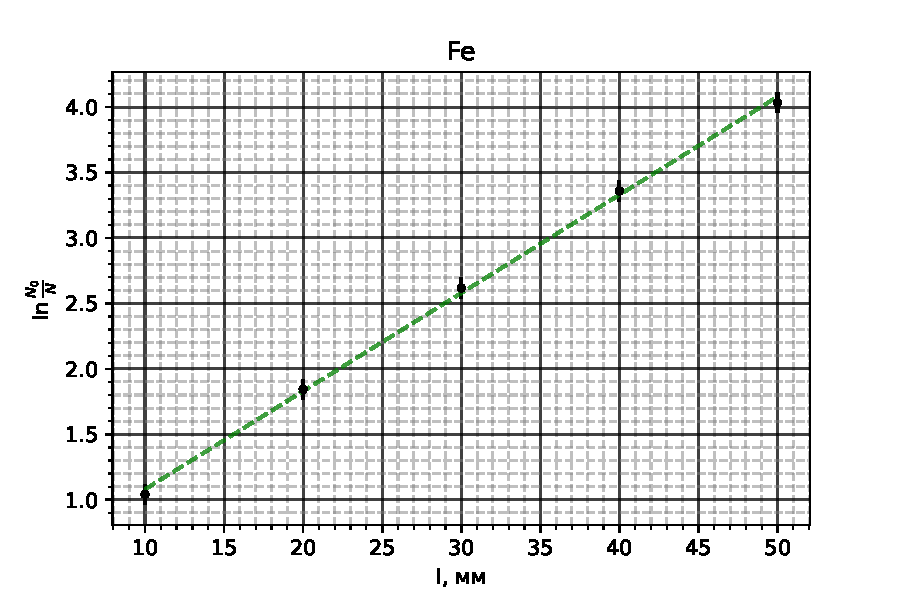
\includegraphics[width=\textwidth]{Fe.pdf}
        \caption{График для железа}
        \label{fig:Fe}
    \end{figure}

    \begin{figure}
        \centering
        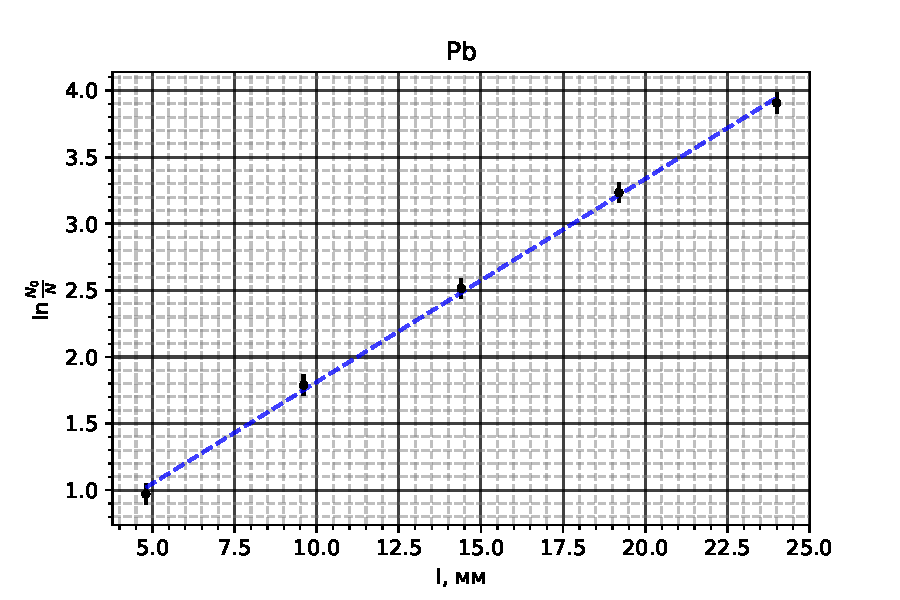
\includegraphics[width=\textwidth]{Pb.pdf}
        \caption{График для свинца}
        \label{fig:Pb}
    \end{figure}

    \begin{figure}
        \centering
        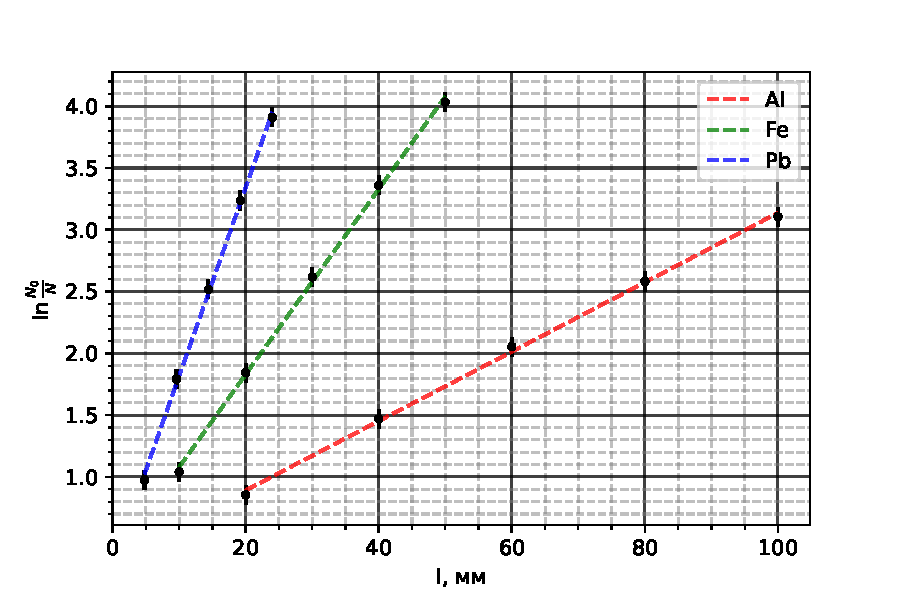
\includegraphics[width=\textwidth]{AlFePb.pdf}
        \caption{График сравнения}
        \label{fig:comparing}
    \end{figure}

    Как видно из графика \ref{fig:comparing}, свинец имеет самую высокую задержку. Это подтверждает следующий график:
    
    \begin{figure}
        \centering
        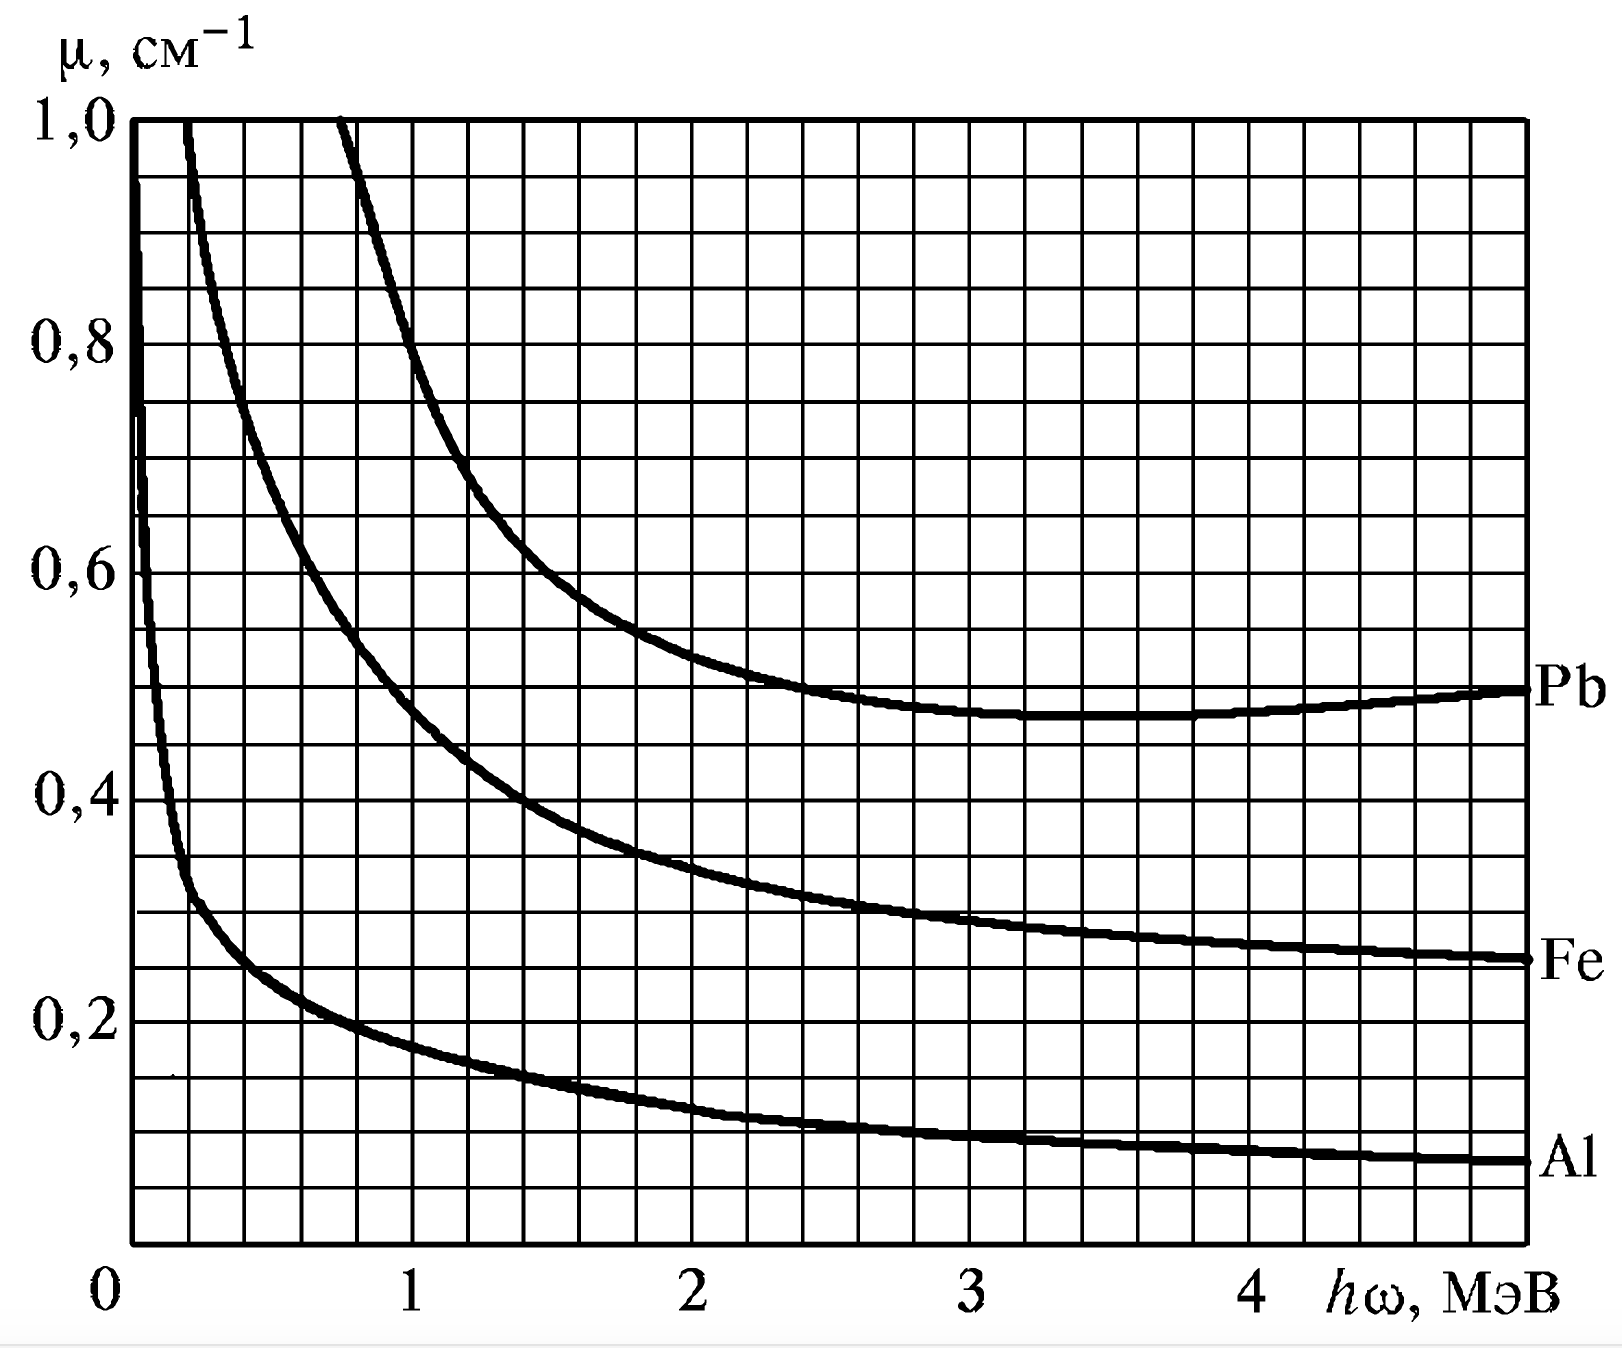
\includegraphics[width=0.5\textwidth]{mu.png}
    \end{figure}

    Запишем коэффициенты $\mu$ для всех метеллов:

    \begin{center}
        $\mu_{Al}$ = (280.74 $\pm$ 5.92) $\cdot 10^{-3}$ см$^{-1}$ \\
        $\mu_{Fe}$ = (749.81 $\pm$ 14.28) $\cdot 10^{-3}$ см$^{-1}$ \\
        $\mu_{Pb}$ = (1524.98 $\pm$ 31.10) $\cdot 10^{-3}$ см$^{-1}$ \\
    \end{center}

    Используя найденные коэффициенты ослабления по таблице определим среднюю энергию
    $\gamma$-лучей, испускаемых источником.

    Воспользовавшись таблицей, определим энергию $\gamma$-кванта.

    \begin{center}
        по Al $E \approx 0.3$ МэВ \\
        по Fe $E \approx 0.4$ МэВ \\
        по Pb $E \approx 0.5 - 0.6$ МэВ \\
    \end{center}

\end{document}